\documentclass[11pt,compress,t,notes=noshow, aspectratio=169, xcolor=table]{beamer}

\usepackage{../../style/lmu-lecture}
% Defines macros and environments
% This file is included in slides and exercises

% Rarely used fontstyle for R packages, used only in 
% - forests/slides-forests-benchmark.tex
% - exercises/single-exercises/methods_l_1.Rnw
% - slides/cart/attic/slides_extra_trees.Rnw
\newcommand{\pkg}[1]{{\fontseries{b}\selectfont #1}}

% Spacing helpers, used often (mostly in exercises for \dlz)
\newcommand{\lz}{\vspace{0.5cm}} % vertical space (used often in slides)
\newcommand{\dlz}{\vspace{1cm}}  % double vertical space (used often in exercises, never in slides)
\newcommand{\oneliner}[1] % Oneliner for important statements, used e.g. in iml, algods
{\begin{block}{}\begin{center}\begin{Large}#1\end{Large}\end{center}\end{block}}

% Don't know if this is used or needed, remove?
% textcolor that works in mathmode
% https://tex.stackexchange.com/a/261480
% Used e.g. in forests/slides-forests-bagging.tex
% [...] \textcolor{blue}{\tfrac{1}{M}\sum^M_{m} [...]
% \makeatletter
% \renewcommand*{\@textcolor}[3]{%
%   \protect\leavevmode
%   \begingroup
%     \color#1{#2}#3%
%   \endgroup
% }
% \makeatother




\title{Interpretable Machine Learning}
% \author{LMU}
%\institute{\href{https://compstat-lmu.github.io/lecture_iml/}{compstat-lmu.github.io/lecture\_iml}}
\date{}

%\bibliography{feature-importance}
%\usepackage{Sweave}
\begin{document}
	\newcommand{\titlefigure}{figure_man/pimp}
    \newcommand{\learninggoals}{
    	\item Understand PIMP and its motivation
            \item Address multiple testing in feature importance}
	% Set style/preamble.Rnw as parent.
	
	% Load all R packages and set up knitr
	
	% This file loads R packages, configures knitr options and sets preamble.Rnw as 
	% parent file
	% IF YOU MODIFY THIS, PLZ ALSO MODIFY setup.Rmd ACCORDINGLY...
	
	% Defines macros and environments

	\lecturechapter{PIMP}
	\lecture{Interpretable Machine Learning}
	
	% ------------------------------------------------------------------------------


\begin{frame}{Testing Importance (PIMP) \citebutton{Altmann et al. (2010)}{https://doi.org/10.1093/bioinformatics/btq134}}

\begin{itemize}[<+->]
  \item PIMP was originally introduced for random forest's built-in PFI scores
  %\item It fixes the problem that the importance measure prefers features with many categories.
  \item PIMP investigates whether the PFI score \textbf{significantly} differs from 0\\
  $\Rightarrow$ Addresses random fluctuations that cause non-zero PFI scores
  %Useful because PFI can be non-zero due to randomness/stochasticity
  \item PIMP tests the $H_0$-hypothesis: Feature is independent of target $y$ (unimportant)
  %It computes the distribution of importances under the $H_0$-hypothesis that the feature is independent of the target $y$
  \item Sampling under $H_0$: Permute target $y$, retrain model, compute PFI scores, repeat\\
  $\Rightarrow$ Permuting $y$ breaks relationship to all features\\
  $\Rightarrow$ By computing PFI scores again, we obtain distribution of PFI scores under $H_0$
  \item %We now rescale the importance to a 
  Compute p-value (tail probability under $H_0$) and use this as new importance measure
\end{itemize}

%\footnote[frame]{\fullcite{altmann2010permutation}}
%{\tiny{Altmann, André, et al. "Permutation importance: a corrected feature importance measure." 
%Bioinformatics 26.10 (2010): 1340-134.}}

\end{frame}

\begin{frame}{Testing Importance (PIMP)}

PIMP algorithm:
\begin{enumerate}
	\item<1-3> For $m \in \{1, \ldots, n_{repetitions}\}$:
		\begin{itemize}
			\item Permute response vector $y$
			\item Retrain model with data $\Xmat$ and permuted $y$
			\item Compute feature importance $PFI_j^m$ for each feature $j$ (under $H_0$)
		\end{itemize}
	\item<2-3> Train model with $\Xmat$ and unpermuted $y$
	\item<3> For each feature $j \in \{1,\ldots,p\}$:
		\begin{itemize}
			\item Fit probability distribution of the feature importance values $PFI_j^m$, $m \in \{1, \ldots, n_{repetitions}\}$ (choice between Gaussian, lognormal, gamma or non-parametric)
			\item Compute feature importance $PFI_j$ for the model without permutation of $y$ (under $H_1$)
			\item Retrieve the p-value of $PFI_j$ based on the fitted distribution
		\end{itemize}
\end{enumerate}
\end{frame}


%TODO: Simplify or better explain example
\begin{frame}{PIMP for extrapolation example}
\textbf{Recall:} 
$y = x_3 + \epsilon_y$ with $\epsilon_y \sim N(0, 0.1)$, 
$x_1$, $x_2$ highly correlated but independent of $y$, 
$x_4$ is independent of $y$ and all other variables.
Fitting a LM yields $\fh(\xv) \approx 0.3 x_1 - 0.3 x_2 + x_3$.
%Fitting a \texttt{lm} yields $\fh(x) \approx 0.3 x_1 - 0.3 x_2 + x_3$.
%
%\begin{figure}
  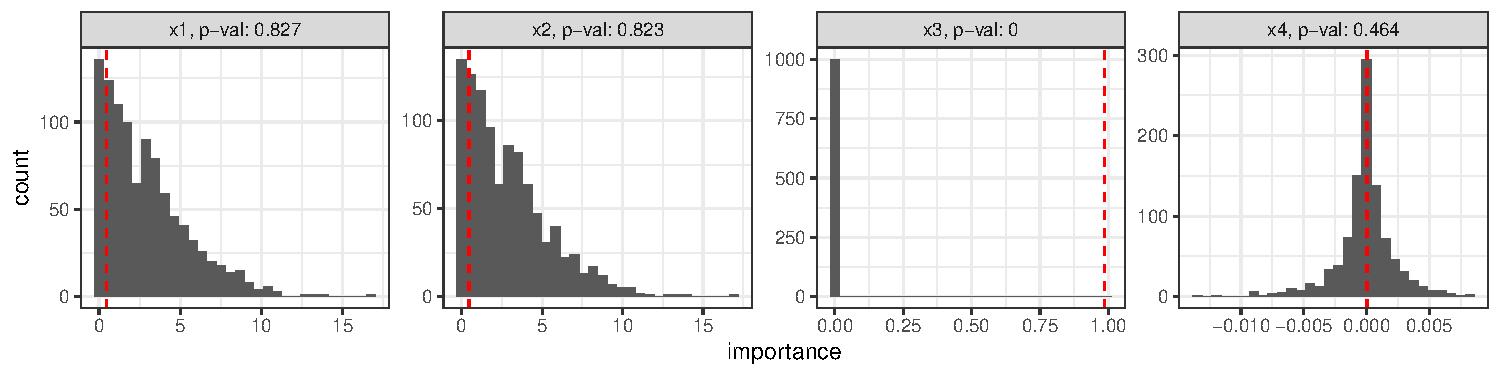
\includegraphics[width=\linewidth]{figure_man/pimp.pdf}
  %\caption{$H_0$ distribution (1000 samples) for each feature as histograms, the true PFI indicated in red. PIMP only considers $x_3$ relevant. Although PFI for $x_1$ and $x_2$ is nonzero, PIMP considers them irrelevant since they are not predictive of $y$. Even after permuting $y$, the model relies on them.}
%\end{figure}

\begin{itemize}
    \item Histograms: $H_0$ distribution of PFI scores after permuting $y$ (1000 repetitions)
    \item Red: PFI score estimated on unpermuted $y$ (under $H_1$) $\leadsto$ compare against $H_0$ distribution
    \item Results: Although PFI for $x_1$ and $x_2$ is nonzero (red), PIMP considers them not significantly relevant (p-value > 0.05) 
    %since they are not predictive of $y$
\end{itemize}
\end{frame}

\begin{frame}{Digression: Multiple testing problem \citebutton{Romano et al. (2010)}{https://doi.org/10.1057/978-1-349-95121-5_2914-1}}
\begin{itemize}[<+->]
  \item When should we reject the $H_0$-hypothesis for a feature? 
  \item The larger the number of features, the more tests need to be performed by PIMP\\
  $\leadsto$ \textbf{Multiple testing problem}: If multiplicity of tests is not taken into account, the probability that some of the true $H_0$-hypothesis is rejected (type-I error) by chance may be large
  \item Accounting for multiplicity of individual tests can be achieved by controlling an appropriate error rate, e.g., the \textbf{family-wise error rate} (FWE: probability of at least one type-I error)
  \item One classical method to control the FWE is the \textbf{Bonferroni correction} which rejects a null hypothesis if its p-value is smaller than $\alpha/m$ with $m$ as the number of performed parallel tests
  %\item We refer to other lectures or the statistics literature for more details
  \end{itemize} 

  %\footnote[frame]{\fullcite{romano2010multiple}}
  %{\tiny{Romano, J. P., Shaikh, A. M., and Wolf, M. (2010). Multiple Testing. The New Palgrave Dictionary of Economys. \url{https://home.uchicago.edu/~amshaikh/webfiles/palgrave.pdf}}\par}
\end{frame}
% \begin{frame}
%   \printbibliography
% \end{frame}

\endlecture
\end{document}
